\chapter{Tecnologie di interesse}
\label{cap:chapter2}

Questo capitolo si occupa di spiegare il funzionamento dei protocolli standard impiegati durante il tirocinio, con l'obiettivo di comprendere successivamente le scelte progettuali intraprese durante lo sviluppo.
\\Particolare attenzione sarà dedicata agli standard definiti dall'Open Geospatial Consortium (OGC), tra cui Web Map Service (WMS), il Web Map Tiles Service (WMTS), Web Feature Service (WFS) e dall'Open Source Geospatial Foundation (OSGEO) tramite il protocollo Tile Map Service (TMS).
\\Si tratta di protocolli universalmente riconosciuti per la distribuzione e l'accesso ai dati geospaziali tramite Internet. Saranno infine analizzate altre tecnologie rilevanti per la gestione e la visualizzazione di dati geospaziali (come GeoJSON e ShapeFile), formati comuni per lo scambio di dati geografici.

\section{Gli standard forniti da OGC}

Il consorzio Open Geospatial Consortium (OGC) ha definito diversi standard per i servizi web che consentono ai client di accedere e interrogare informazioni geografiche. Tra questi troviamo:
\begin{itemize}
      \item Web Map Service (WMS);
      \item Web Map Tile Service (WMTS);
      \item Web Feature Service (WFS);
\end{itemize}
Ciascuno di questi standard offre funzionalità specifiche per soddisfare diverse esigenze di accesso ai dati geospaziali. Questi servizi si basano su altre tecnologie come l'architettura REST e il protocollo SOAP, che trasmettono i messaggi di risposta ai client in formato XML.
\\Lo standard OGC prevede che tutti i client che necessitano di contattare il servizio debbano prima effettuare una richiesta HTTP denominata \textit{GetCapabilities}. Questa operazione è necessaria, per il client, per poter sapere quali informazioni possono essere reperite da quel servizio. In generale, queste informazioni comprendono: le mappe (una o più), le proiezioni che supportano, i loro confini (bounding box), i loro formati (PNG, JPG, GML) e le altre richieste HTTP che si possono fare al servizio stesso.

\subsection{Protocollo WMS}

Il Web Map Service (WMS) è universalmente riconosciuto come uno dei principali standard nel contesto dei servizi geospaziali, ed è tra i più importanti per la distribuzione di dati di mappe attraverso la rete Internet.
Questo protocollo si occupa di offrire una rappresentazione visiva delle mappe geografiche, distribuendole essenzialmente sotto forma di immagini raster, come PNG o JPG, ma possono anche essere trasmesse in un formato vettoriale come SVG.
\\In conformità agli standard, quando un client desidera contattare un server WMS, la prima operazione che viene eseguita è una richiesta di GetCapabilities. La risposta a tale richiesta contiene principalmente: l'elenco di tutte le mappe disponibili, denominate \textit{Layer}; l'elenco di tutte le proiezioni supportate e il formato immagine in cui la mappa può essere restituita. Una volta ricevute queste informazioni, il client, dopo aver scelto il layer da visualizzare, invia una richiesta di GetMap al server, specificando i parametri necessari per visualizzare l'immagine richiesta. Tra questi parametri, è incluso il Bounding Box che serve per definire l'area geografica della mappa che si vuole visualizzare. Il server, a sua volta, risponde inviando l'immagine della mappa che contiene l'area specificata nei Bounding Box.
\\Inoltre, lo standard WMS supporta anche la trasparenza delle immagini restituite nelle richieste, permettendo così la sovrapposizione visiva e la combinazione di più layer forniti da server geospaziali. Infine, se abilitato, consente agli utenti di ottenere informazioni specifiche su determinate caratteristiche presenti sulla mappa, come punti di interesse o dati geografici particolari.
\begin{figure}[htbp]
      \centering
      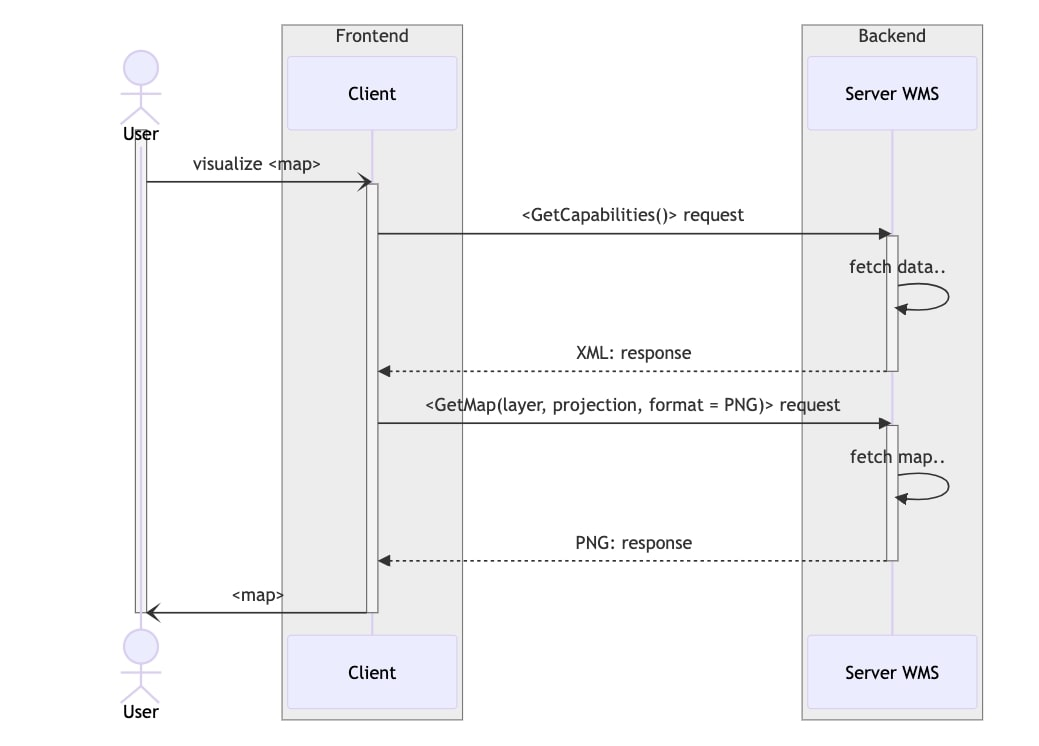
\includegraphics[width=1\textwidth]{images/Capitolo2/ProtocolWMS.jpg}
      \caption{Diagramma di Sequenza del protocollo WMS}
      \label{fig:wms protocol}
\end{figure}

\subsubsection{Formato della richiesta}

Lo standard specifica diversi tipi di richieste che possono essere effettuate ai server WMS:
\begin{itemize}
      \item \textit{GetCapabilities}: questa richiesta restituisce un documento XML che rappresenta le informazioni sul servizio WMS stesso. Nello specifico, fornisce l'elenco dei layer disponibili, le proiezioni supportate, i bounding box (rispettivi per ogni proiezione), la versione del protocollo WMS supportata, gli stili delle mappe disponibili e un abstract che fornisce una descrizione della mappa.     
      \item \textit{GetMap}: utilizzata per ottenere un'immagine di mappa dal servizio. I parametri inclusi nella richiesta comprendono: il nome del layer, la versione del protocollo utilizzato, lo stile, la proiezione, i bounding box, il formato e la larghezza e altezza dell'immagine in pixel. La risposta alla richiesta è un'immagine della mappa, pronta per essere visualizzata su un browser web o in un'applicazione client.
\end{itemize}
I tipi di richiesta che i fornitori di WMS possono opzionalmente supportare includono:
\begin{itemize}
      \item \textit{GetFeatureInfo}: consente di ottenere informazioni dettagliate su specifiche caratteristiche presenti sulla mappa. Restituisce informazioni associate a quella posizione, come punti di interesse o dati geografici particolari.
      \item \textit{DescribeLayer}: restituisce i tipi di feature disponibili per i layer specificati, che possono essere ulteriormente descritti utilizzando richieste Web Feature Service (WFS). Questa richiesta è utile per comprendere meglio la struttura e le caratteristiche dei dati geospaziali presenti nel servizio WMS.
      \item \textit{GetLegendGraphic}: utilizzata per ottenere un'immagine della legenda della mappa, questa richiesta fornisce una guida visiva agli elementi presenti sulla mappa, come i simboli e le etichette dei layer.
\end{itemize}
Qui sotto è riportato uno snippet che contiene alcuni esempi possibili di richieste WMS, eseguite utilizzando il comando cURL per simulare il comportamento di una richiesta HTTP.
\lstinputlisting[language=bash]{listings/Capitolo2/wms-requests-example.sh}
Qui di seguito invece viene mostrato al lettore un esempio di richiesta funzionante, fatta durante il percorso di tirocinio, ai server WMS del Geoportale Nazionale, gestito dal Ministero dell'Ambiente e della Sicurezza Energetica.
Ciò serve per ottenere dati geospaziali relativi alla mappa che illustra l'area allagabile conforme al Piano di Gestione del Rischio di Alluvioni (PGRA) del 2021.
\lstinputlisting[language=bash]{listings/Capitolo2/wms-requests.sh}
Come si può vedere dal messaggio di risposta \cite{GetCapabilitiesWMS} in formato XML inviato dai loro Server,
il servizio offre funzionalità standard come la richiesta di mappe (GetMap) e informazioni (GetFeatureInfo), oltre a supportare la descrizione dei layer (DescribeLayer) e la visualizzazione della legenda (GetLegendGraphic).
\\Per ulteriori informazioni dettagliate sullo standard WMS, è possibile fare riferimento alla documentazione ufficiale disponibile sul sito web di Open Geospatial Consortium \cite{DocumentazioneWMS}

\subsection{Protocollo WMTS}

A differenza del WMS, il quale invia un'unica immagine per ogni mappa ai client, il WMTS la "segmenta" in piccole porzioni rettangolari, denominate \textit{tiles}. Queste ultime vengono prima pre-renderizzate e poi memorizzate sul server. Successivamente, sotto richiesta dei client, vengono recuperate e restituite come messaggio di risposta. 
\\Nello specifico, quando un client desidera visualizzare una mappa, invia al server WMTS tante richieste HTTP differenti per ogni tiles che vuole ottenere. Ciascuna richiesta contiene al suo interno: la porzione di mappa, la proiezione e il formato di immagine desiderato. Il server, per ogni richiesta HTTP ricevuta, risponde di conseguenza, inviando al client le tiles. A questo punto il client, una volta ottenute le tiles, le combina insieme per formare la porzione di immagine di mappa richiesta.
\\Una delle principali caratteristiche del WMTS è che l'utilizzo delle tiles riduce la quantità di elaborazione necessaria al server per mostrare correttamente la mappa. Il server WMTS deve infatti fornire solo le tiles necessarie per l'area richiesta e può riutilizzare parti di mappa già calcolate in precedenza, anziché generare e inviare tutte le volte un'unica immagine completa.
\\Inoltre, l'utilizzo di tiles facilita l'implementazione di una politica di caching, in quanto essendo piccole porzioni di immagini, queste possono essere memorizzate facilmente. Sul lato back-end, infatti, il servizio WMTS può memorizzare nella cache le tiles più utilizzate e restituirle più rapidamente al client. Lato front-end, invece, il browser è in grado di intercettare le risposte inviate dal server e di memorizzare nella sua cache interna l'immagine della tile. In questo modo, quando il client richiede la stessa tile, quest'ultima viene visualizzata senza dover contattare nuovamente il server. Diversamente, nel protocollo WMS, risulta essere più complesso implementare il meccanismo di caching a causa dei parametri che vengono utilizzati nelle richieste di GetMap. I query params di tale richiesta, infatti, risultano essere molto più variabili, specialmente con il parametro Bounding Box che cambia ogni qualvolta che si visualizza una porzione geografica differente.

\begin{figure}[htbp]
      \centering
      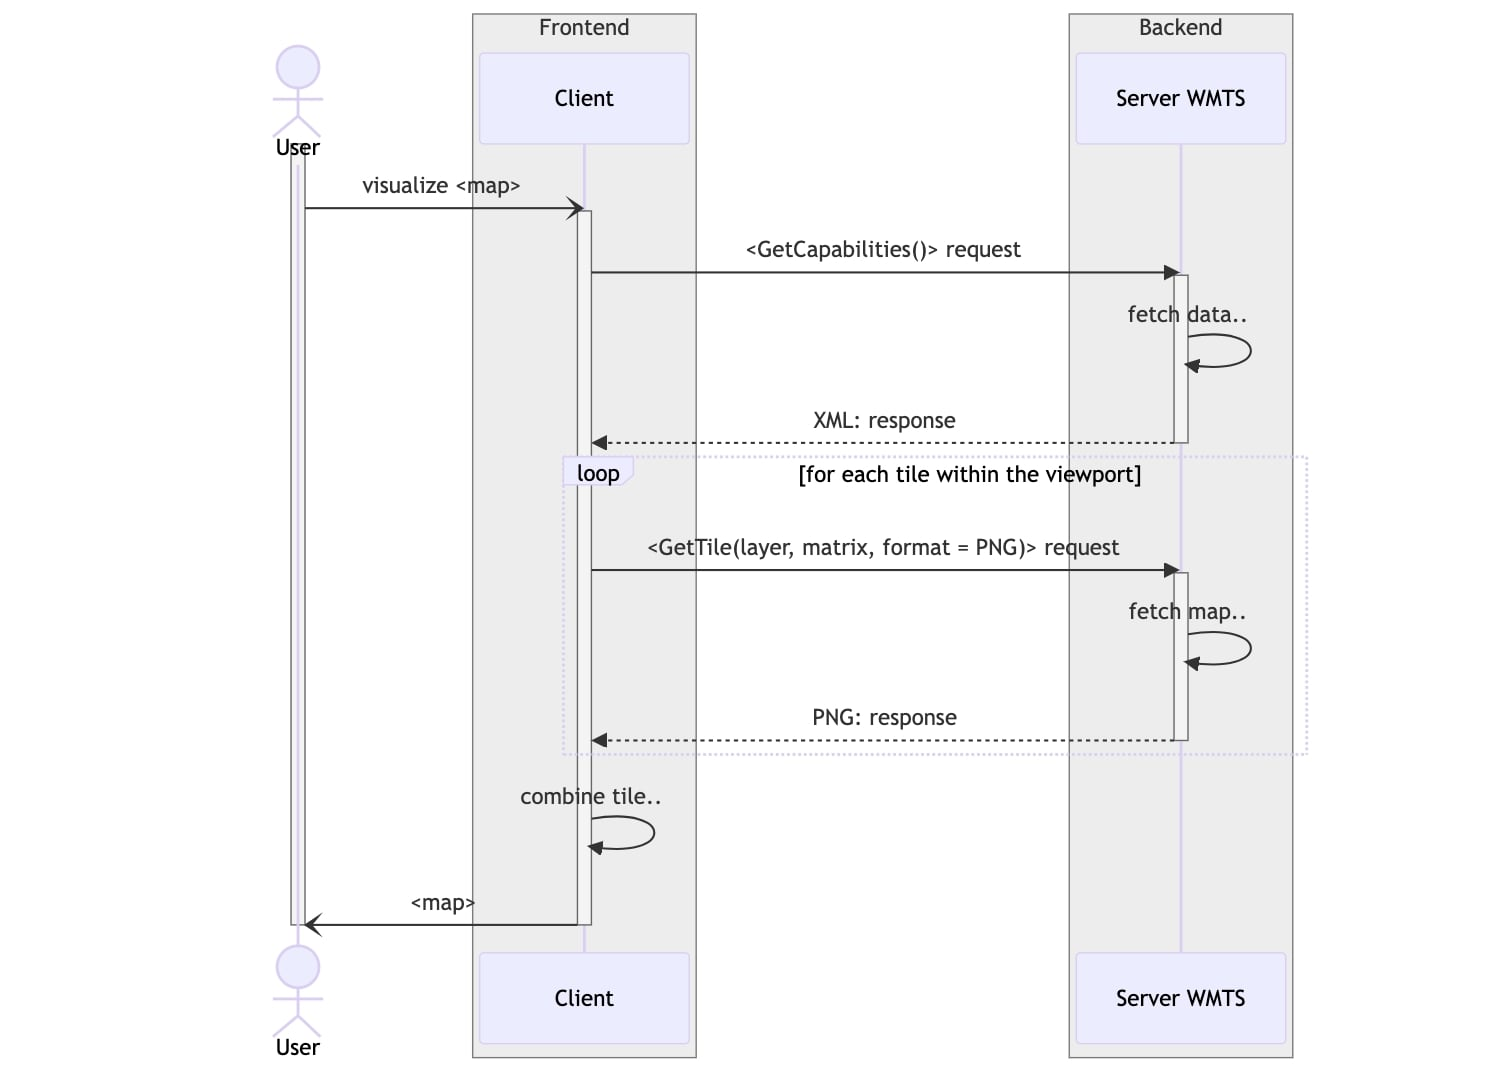
\includegraphics[width=1\textwidth]{images/Capitolo2/ProtocolWMTS.jpg}
      \caption{Diagramma di Sequenza del protocollo WMTS}
      \label{fig:wmts protocol}
\end{figure}

\subsubsection{Formato della richiesta}

\begin{itemize}
      \item \textit{GetCapabilities}: Restituisce un documento XML che descrive il \textit{Manifest} del servizio WMTS, inclusi i layers disponibili, i formati supportati, le coordinate di riferimento e altro ancora.
      \item \textit{GetTile}: Restituisce una Tile specifica in base alle coordinate geografiche e allo zoom specificato nella richiesta.
      \item \textit{GetFeatureInfo}: Questa richiesta non è molto comune nei servizi WMTS, in quanto generalmente viene direttamente utilizzata la richiesta GetFeatureInfo fornita dal servizio WMS. Se abilitata, questa richiesta restituisce informazioni aggiuntive associate a una tile, come attributi dei dati geospaziali presenti in quel punto della mappa.
\end{itemize}
Qui di seguito è riportato uno \textit{snippet} contenente alcuni esempi possibili di richieste WMTS, eseguite utilizzando il comando cURL per simulare il comportamento di una richiesta HTTP.

\lstinputlisting[language=bash]{listings/Capitolo2/wmts-requests-example.sh}
Per ulteriori informazioni dettagliate sullo standard WMTS, è possibile fare riferimento alla documentazione ufficiale disponibile sul sito web di Open Geospatial Consortium \cite{DocumentazioneWMTS}

\subsection{Protocollo WFS}

Il Web Feature Service (WFS) è un servizio web utilizzato per accedere e manipolare dati geospaziali attraverso internet. La differenza principale tra un servizio WMS e WFS risiede nel tipo di dati che vengono trasmessi e nel modo in cui vengono rappresentati dal client.
\\Come già spiegato, il servizio WMS si occupa principalmente di offrire una rappresentazione visiva delle informazioni geografiche, distribuendo le mappe principalmente sotto forma di immagini raster o vettoriali. Quest'ultime sono già pronte per essere visualizzate e non richiedono ulteriori elaborazioni: il client dovrà soltanto rappresentarle nella corretta proiezione.
\\Un WFS trasmette dati geospaziali grezzi, come numeri, coordinate e altre proprietà, che devono essere interpretati e visualizzati dal client. Ciò significa che sarà compito del client elaborare questi dati e rappresentarli come mappa con uno specifico stile grafico, disegnando ad esempio punti, linee o poligoni secondo le specifiche della visualizzazione desiderata. Tali dati, che prendono il nome di "Feature", sono dati geospaziali vettoriali che vanno a rappresentare oggetti geografici reali come per esempio strade, fiumi o frane. Ogni feature possiede al proprio interno un insieme di attributi che definiscono il suo tipo di geometria e la sua posizione sulla mappa. Inoltre, una Feature può includere ulteriori proprietà che forniscono più informazioni sulla feature stessa, come ad esempio: nome, altezza, larghezza, regione, etc...
\\Per comprendere meglio la differenza, qui di seguito è riportato un esempio Feature, nel formato geospaziale GeoJSON che è stato utilizzato durante il tirocinio.
\lstinputlisting[language=JSON]{listings/Capitolo2/exampleGeoJson.json}
Similmente al WMS, che attraverso la richiesta GetMap può richiede una mappa specifica al server, il servizio WFS offre la richiesta GetFeature per richiedere una feature precisa che il server WFS provvederà a fornirgli.
\\I client possono anche eseguire operazioni di analisi spaziale, come il calcolo dell'area di un poligono o la ricerca delle feature più vicine a una determinata posizione.
Ad esempio, è possibile interrogare il servizio per ottenere informazioni su tutti gli edifici situati in una determinata area, oppure trovare tutti i fiumi di una certa lunghezza.
\\Queste informazioni vengono trasmesse utilizzando il formato GML (Geography Markup Language), ovvero un formato basato su XML che consente di descrivere in modo dettagliato la geometria e le proprietà di ciascuna feature. Ciò non toglie che i servizi WFS possano supportare anche altri tipi di formati, come il GeoJSON. In questo caso sarà dovere del server, definire all'interno delle informazioni presenti nella richiesta di GetCapabilities, tutti i formati geospaziali supportati. A quel punto il client, potrà richiedere il tipo di formato desiderato specificandolo nei queryParams (per esempio \textit{outputFormat=application/json}).

\begin{figure}[htbp]
      \centering
      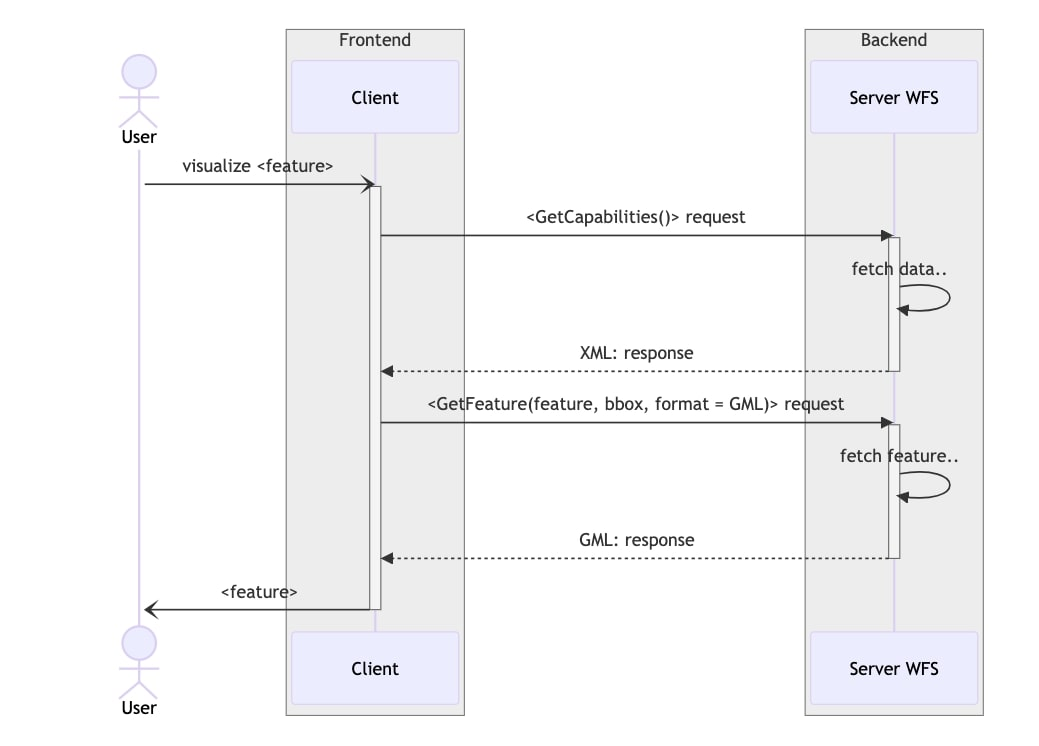
\includegraphics[width=1\textwidth]{images/Capitolo2/ProtocolWFS.jpg}
      \caption{Diagramma di Sequenza del protocollo WFS}
      \label{fig:wfs protocol}
\end{figure}

\subsubsection{Formato della richiesta}

Le richieste che è possibile fare a un servizio WFS (Web Feature Service) sono le seguenti:

\begin{itemize}
      \item \textit{GetCapabilities}: Come per i WMS, la richiesta GetCapabilities restituisce un documento XML che fornisce informazioni dettagliate sul servizio WFS stesso. Queste informazioni includono i tipi di feature disponibili, i formati di trasmissione dei dati supportati (GML, GeoJSON, ecc..), i tipi di richieste supportate, le proiezioni geografiche disponibili e altre capacità del servizio.
      \item \textit{GetFeature}: è la richiesta principale nel protocollo WFS in quanto consente agli utenti di recuperare la feature interessata. I parametri inclusi nella richiesta comprendono il nome della feature, il tipo di formato desiderato, la sua proiezione, ecc..
      \item \textit{DescribeFeatureType}: è usata per richiede informazioni su un singolo tipo di feature prima di chiedere effettivamente la feature stessa. In particolare, l'operazione richiede un elenco di feature e attributi per il tipo di feature dato, oppure un elenco dei tipi di feature disponibili.
\end{itemize}
I tipi di richiesta che i servizi WFS possono opzionalmente supportare sono:
\begin{itemize}
      \item \textit{Transaction}: consente agli utenti di modificare i dati geografici nel servizio WFS, attraverso le operazioni come inserimento, modifica o eliminazione di una feature. Ciò è utile per gli utenti che hanno bisogno di mantenere aggiornati i dati geografici all'interno del servizio, consentendo loro di interagire direttamente e apportare modifiche in tempo reale.
      \item \textit{GetPropertyValue}: questa richiesta consente agli utenti di ottenere i valori degli attributi di una o più feature, senza recuperarne tutti i dettagli geometrici associati.
      \item \textit{LockFeature}: consente agli utenti di acquisire una lock di accesso in mutua esclusione alla feature, impedendo ad altri utenti di modificarla contemporaneamente.
      \item \textit{GetFeatureWithLock}: questa richiesta combina le funzionalità di GetFeature e LockFeature. In questo modo è possibile acquisire una lock di accesso in mutua esclusione alla feature desiderate prima di richiedere la feature stessa.
\end{itemize}
Qui di seguito è riportato uno \textit{snippet} contenente alcuni esempi possibili di richieste WFS, eseguite utilizzando il comando cURL per simulare il comportamento di una richiesta HTTP.

% \texttt{WFS example requests}.
\lstset{basicstyle=\footnotesize\ttfamily}
\lstinputlisting[language=bash]{listings/Capitolo2/wfs-requests-example.sh}
Ecco un altro esempio di richiesta funzionante, effettuata sempre durante il percorso di tirocinio, ai server WFS del Geoportale Nazionale.
Come si può notare, questa richiesta è simile a quella effettuata precedentemente per il servizio WMS, ma questa volta viene rivolta al servizio WFS. Entrambi i servizi offrono informazioni sulla stessa mappa, ma con approcci diversi: mentre il WMS fornisce immagini della mappa, il WFS trasmette le feature geospaziali che compongono la mappa.

\lstset{basicstyle=\footnotesize\ttfamily}
\lstinputlisting[language=bash]{listings/Capitolo2/wfs-requests.sh}
Anche in questo caso, come si può vedere dal loro messaggio di risposta \cite{GetCapabilitiesWFS} in formato XML inviato dai loro Server,
il servizio offre funzionalità standard come la richiesta di feature (GetFeature) e la descrizione dei tipi di feature (DescribeFeatureType), oltre a supportare la modifica dei dati geografici tramite transazioni (Transaction).
\\Per ulteriori informazioni dettagliate sullo standard WFS, è possibile fare riferimento alla documentazione ufficiale disponibile sul sito web di Open Geospatial Consortium \cite{DocumentazioneWFS}

\section{Tiled Map Service (TMS)}

Il protocollo Tiled Map Service (TMS), è un altro standard utilizzato per servire mappe geospaziali. A differenza di quelli sopra citati, questa specifica non è definita dall'Open Geospatial Consortium, ma è stata introdotta dall'Open Source Geospatial Foundation (OSGeo). Per questo motivo, nonostante entrambi i protocolli si occupano di fornire dati di mappe, presentano delle differenze.
\\Questo standard può essere considerato come una versione più "leggera" del servizio WMTS, in quanto continua a servire mappe sotto forma di tiles, ma offre contemporaneamente meno funzionalità.
Infatti, questo standard non richiede che il client debba prima ottenere informazioni sul servizio attraverso una richiesta simile a GetCapabilities, ma può può dedurre queste informazioni dalla struttura dell'URL stesso. Il client, infatti, può accedere direttamente alle tiles della mappa tramite percorso URL, in cui ogni tiles è rappresentata da un percorso differente.
Si può dunque affermare che la struttura degli URL di un servizio TMS segue una convenzione simile a quella delle cartelle: ogni livello di zoom della mappa e ogni tile è rappresentata da un URL univoco e questi possono essere organizzati in modo gerarchico, nello stesso modo delle cartelle in un File System.
\\Questo comporta da un lato un protocollo più semplice, ma dall'altro meno funzionalità: ad esempio, il servizio non può fornire informazioni su tutti i tipi di richieste a cui può essere interrogato. Nel caso di un servizio WMS, il client attraverso GetCapabilities può capire o meno se il server supporta ulteriori richieste come GetFeatureInfo o GetLegendGraphic.
Inoltre, il protocollo TMS prevede solo la trasmissioni di immagini tile, non restituisce altri tipi di informazioni (come nel caso della GetLegendGraphic che restituisce l'immagine della legenda associata allo stile della mappa).
\\Ciò può sembrare una cosa negativa, ma è importante tenere conto anche del peso delle richieste. Una richiesta di GetCapabilities ad un servizio di mappe può restituire un messaggio di risposta molto grande e pesante, sopratutto se contiene molti layer (mappe) al suo interno. Durante il tirocinio è capitato per esempio di ricevere risposte di un peso oltre i 30MB. Anche se può sembrare insignificante, gestire un peso simile all'interno di servizi web risulta molto tedioso, specialmente dal punto di vista della memorizzazione nella cache del browser.
\\Inoltre, avere una struttura gerarchica simile a quella di un File System, può portare a tanti benefici. Uno di essi, ad esempio, è la facilità nel distribuire tutte le tiles tramite una CDN (Content Delivery Network) in modo elementare. La stessa cosa può essere fatta anche nel caso dei servizi WMTS tramite query params, ma risulta molto più complesso e difficile da gestire.
Utilizzando il protocollo TMS, infatti, è possibile archiviare le tiles in uno storage generico e servirle senza la necessità di elaborare nuovamente le richieste in ingresso. Ad esempio, su AWS, questa operazione può essere eseguita utilizzando lo storage S3 e la CDN CloudFront, entrambi privi di meccanismi specifici per la gestione dei dati o dei protocolli GIS. Questo approccio consente un miglior bilanciamento del carico sul server, permette di offrire la stessa mappa su più istanze contemporaneamente e garantisce la continuità del servizio.
\\Infine, le richieste di un servizio TMS sono più facili da memorizzare nella cache del browser rispetto al WMTS perché i suoi URL sono semplici e diretti. Al contrario, il WMTS spesso utilizza parametri più complessi nelle sue richieste, attraverso l'utilizzo dei query parameters, rendendo la memorizzazione nella cache del browser meno diretta e più soggetta a variazioni.
\\La struttura di una richiesta TMS per accedere ad una specifica tile è la seguente
\lstinputlisting[language=bash]{listings/Capitolo2/tms-requests-example.sh}
Questa richiesta restituisce direttamente una tile della mappa, generalmente grande 256x256, nel formato e proiezione richiesti. Le coordinate x e y rappresentano la posizione della tile all'interno della griglia, mentre la z il suo livello di zoom. Per ogni livello di zoom sono presenti dei confini, chiamati "Bounding Box" o "extent" che indicano l'estensione geografica delle tiles disponibili per quel livello di zoom. Se vengono richieste delle tile al di fuori di questi confini, il server TMS restituisce ovviamente un messaggio di errore.
\begin{figure}[htbp]
      \centering
      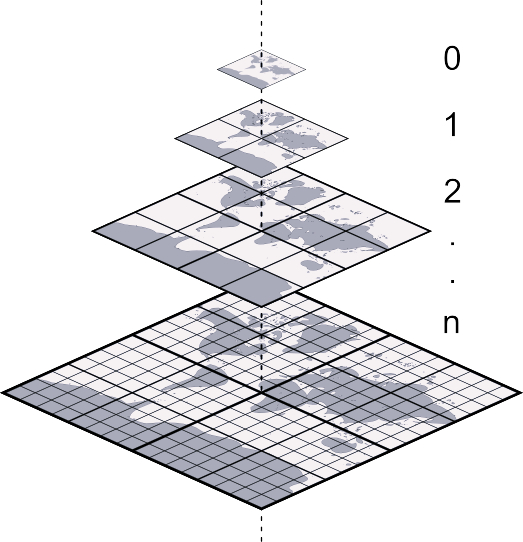
\includegraphics[width=0.5\textwidth]{images/Capitolo2/tilesPyramid.jpg}
      \caption{Tiles con livello di zoom}
      \label{fig:tmsTiles}
\end{figure}

\subsubsection{Formato della richiesta}

Come indicato nella specificata del servizio TMS \cite{DocumentazioneTMS}, esistono anche altre richieste che un client può effettuare per ottenere ulteriori informazioni oltre a quella relativa alle tiles. Le principali sono:
\begin{itemize}
      \item \textit{TileMapServiceResource}: questa richiesta è quella più simile a GetCapabilities, permette di vedere tutte le mappe disponibili che il servizio TMS ha a disposizione, specificando il nome della mappa, il formato dell'immagine e la sua proiezione. Può anche essere fornita più volte la stessa mappa, con formati e proiezioni differenti. Un esempio di risposta a tale richiesta è la seguente:
            \lstset{basicstyle=\footnotesize\ttfamily}
            \lstinputlisting[language=xml]{listings/Capitolo2/TileMapServiceResource.xml}
      \item \textit{TileMapResource}: questa richiesta fornisce informazioni più dettagliate su una mappa, specificandone i confini, la dimensione delle tile, la proiezione e tutti i livelli di zoom disponibili che il client può richiedere (coordinata z) con i suoi rispettivi confini (extent). Un esempio di risposta a tale richiesta è la seguente:
            \lstset{basicstyle=\footnotesize\ttfamily}
            \lstinputlisting[language=xml]{listings/Capitolo2/TileMapResource.xml}
      \item \textit{TileResource}: la richiesta effettiva per richiedere la tile che corrispondete esattamente a quella spiegata in precedenza.
\end{itemize}
Il ciclo di vita di un client che richiede una mappa da un server TMS può essere descritto nel seguente modo:
inizialmente, il client contatta tramite richiesta TileMapServiceResource un server TMS per ottenere le informazioni di tutte le mappe disponibili.
Dopo aver selezionato la mappa desiderata, il client utilizza la richiesta TileMapResource per ottenere tutti i possibili livelli di zoom, con i relativi confini.
A questo punto il client richiede direttamente le tiles della mappa desiderata attraverso le coordinate x, y e z, senza sforare dai confini. Il server risponde risponde con l'immagine della tile.

\section{Formati di file Geospaziali}
I formati di file geospaziali sono tipi di file che vengono utilizzati per memorizzare e scambiare dati geografici. Questi dati possono includere informazioni come mappe, immagini satellitari, dati di altitudine, di utilizzo del suolo e molti altri. Alcuni dei formati di file geospaziali più comuni includono:
\begin{itemize}
      \item \textit {Shapefile} (.shp): è uno dei formati più diffusi per memorizzare dati geografici vettoriali, come punti, linee e poligoni.
      \item \textit {GeoTIFF} (.tif): è una versione del formato di file di immagini TIFF (Tagged Image File Format) e viene usato per rappresentare principalmente immagini raster geografiche.
      \item \textit {GeoJSON} (.json): è un formato di file basato su JSON (JavaScript Object Notation) e similmente allo Shapefile, è utilizzato per memorizzare dati geografici vettoriali. Questo formato è spesso utilizzato per lo scambio di dati geografici tramite protocollo HTTP.
      \item \textit {KML/KMZ} (.kml, .kmz): KML (Keyhole Markup Language) è un formato di file XML utilizzato per memorizzare dati geografici ed ha una sua versione compressa nota con il nome di KMZ.
      \item \textit {GeoPackage} (.gpkg): è un formato che memorizza i dati geospaziali utilizzando il linguaggio SQL per gestire e interrogare i dati contenuti al suo interno, sia vettoriali che raster.
\end{itemize}
La diversità di formati esistenti non costituisce un problema per i client che necessitano di utilizzare dati geospaziali. 
Normalmente, si tende a conservare sui server i dati di mappe nei formati sopra citati. 
\\Un server di mappe, a sua volta, può quindi supportare contemporaneamente più servizi (WMS, WMTS, WFS, TMS, etc...).  Questo perché ciascun server di mappe è in grado di convertire gli stessi dati iniziali in formati diversi, solitamente quelli richiesti dai client attraverso il protocollo da loro scelto.
\\Ad esempio, un server WMS permette di richiedere una mappa in formato PNG o JPG. Quando viene effettuata una richiesta tramite questo servizio, il server accede ai suoi dati, ad esempio degli Shapefile, li converte nel formato specificato (PNG o JPG) e li restituisce al client che li aveva richiesti.
È da notare come non ci si debba necessariamente attenere ad uno dei protocolli standard esistenti, ma si possa anche specificarne uno personalizzato che permetta di restituire i dati iniziali in un formato scelto a proprio piacimento. Ad esempio, si potrebbe realizzare un protocollo che restituisce i dati direttamente nel loro formato originario.

\section{Software utilizzati}

L'integrazione dei protocolli OGC è stata resa possibile mediante l'utilizzo di due tecnologie distinte, le quali hanno svolto un ruolo specifico all'interno del progetto di tirocinio.
\\Per la parte di sviluppo front-end, si è fatto uso di OpenLayers, una libreria JavaScript che permette di realizzare interfacce grafiche per la visualizzazione di mappe geospaziali. Quest'ultima offre, in maniera basilare, una mappa interattiva con delle funzionalità già implementate, come ad esempio lo zoom e l'interazione con elementi a schermo, e delle API ad alto livello, che permettono di utilizzare i protocolli sopra menzionati. Un'analisi dettagliata sull'implementazione di questa libreria e le motivazioni che hanno portato alla sua adozione all'interno del progetto, sono approfondite nel capitolo \ref{cap:chapter4}.
\\Fra tutti gli elementi componenti il back-end invece, al fine di risolvere alcuni problemi implementativi riscontrati durante il tirocinio, è stato introdotto un nuovo software, denominato GeoServer. Quest'ultimo permette di memorizzare al suo interno, anche se in maniera laboriosa e complessa, dati di mappe geospaziali e permette di servirli utilizzando i protocolli appena descritti. Le scelte che hanno portato al suo impiego e il suo funzionamento sono approfondite nel capitolo \ref{cap:chapter5}. La modalità con cui viene risolta la complessità legata all'inserimento delle mappe, invece, viene spiegata nel capitolo \ref{cap:chapter6}.
